\documentclass[12pt,a4paper]{article}

\usepackage[utf8]{inputenc}
\usepackage[T1]{fontenc}
\usepackage{geometry}
\usepackage{hyperref}
\usepackage{graphicx}
\usepackage{booktabs}
\usepackage{array}
\usepackage{listings}
\usepackage{xcolor}
\usepackage{enumitem}
\usepackage{setspace}

\geometry{left=2cm,right=2cm,top=2cm,bottom=2cm}
\onehalfspacing
\graphicspath{{report/images/}{images/}}

\definecolor{codegray}{rgb}{0.95,0.95,0.95}
\definecolor{codeblue}{rgb}{0.1,0.1,0.6}

\lstset{
    backgroundcolor=\color{codegray},
    basicstyle=\ttfamily\small,
    keywordstyle=\color{codeblue}\bfseries,
    commentstyle=\color{gray},
    stringstyle=\color{red!60!black},
    breaklines=true,
    frame=single,
    numbers=left,
    numberstyle=\tiny,
    tabsize=4,
    showstringspaces=false
}

\begin{document}

\begin{titlepage}
    \centering
    \vspace*{2cm}

    {\Large Machine Learning Project Documentation\par}
    \vspace{1.5cm}

    {\Huge\bfseries Steam Game Success Predictor\par}
    \vspace{0.5cm}

    {\Large KNN, SVM, Random Forest and Deep Learning\par}

    \vfill

    \begin{flushleft}
    \textbf{Student:} Your Name \\
    \textbf{Course:} Machine Learning \\
    \textbf{Instructor:} Instructor Name \\
    \textbf{Project:} Steam Game Success Prediction \\
    \textbf{Type:} Binary Classification \\
    \textbf{Tools:} Python, Scikit-learn, TensorFlow/Keras, Streamlit \\
    \textbf{Dataset:} Steam Games Dataset
    \end{flushleft}

    \vfill

    {\large \today\par}
\end{titlepage}

\tableofcontents
\newpage

\section{Project Overview}

This project predicts whether a Steam game can be considered successful based on numerical game information. The project uses four different machine learning approaches:

\begin{itemize}[noitemsep]
    \item K-Nearest Neighbors (KNN)
    \item Support Vector Machine (SVM)
    \item Random Forest Classifier
    \item Deep Learning Neural Network
\end{itemize}

Each model is trained and saved separately. A combined Streamlit deployment application is also provided. The combined application allows the user to enter game information once and compare predictions from all four models.

\section{Project Objectives}

The main objectives of this project are:

\begin{itemize}[noitemsep]
    \item to prepare a Steam games dataset for machine learning;
    \item to create a binary target variable representing game success;
    \item to train and compare several classical machine learning models;
    \item to implement a neural network model for the same classification task;
    \item to evaluate model performance using appropriate classification metrics;
    \item to add cross-validation, mean accuracy and standard deviation for model stability analysis;
    \item to deploy the trained models using Streamlit;
    \item to provide screenshots of both the application interface and important implementation code.
\end{itemize}

\section{Project Structure}

\begin{lstlisting}
D:\projects
|-- app.py
|-- KNN_Project
|   |-- app.py
|   |-- steam.csv
|   |-- knn_model.pkl
|   |-- scaler.pkl
|   `-- Untitled.ipynb
|-- SVM_Project
|   |-- app.py
|   |-- steam.csv
|   |-- svm_model.pkl
|   |-- scaler.pkl
|   |-- svm_features.pkl
|   `-- Untitled.ipynb
|-- randomForest
|   |-- app.py
|   |-- steam.csv
|   |-- random_forest_model.pkl
|   |-- rf_features.pkl
|   `-- Untitled1 (1).ipynb
|-- deepLearning
|   |-- app.py
|   |-- steam.csv
|   |-- deep_learning_model.keras
|   |-- dl_scaler.pkl
|   |-- dl_features.pkl
|   |-- deep_learn.ipynb
|   `-- .venv
`-- report
    |-- steam_ml_deep_learning_report.tex
    `-- steam_ml_project_documentation.tex
\end{lstlisting}

\section{Main Files}

\begin{table}[h]
\centering
\begin{tabular}{p{5cm} p{9cm}}
\toprule
\textbf{File} & \textbf{Purpose} \\
\midrule
\texttt{app.py} & Combined Streamlit deployment for all four models. \\
\texttt{KNN\_Project/Untitled.ipynb} & KNN training and evaluation notebook. \\
\texttt{SVM\_Project/Untitled.ipynb} & SVM training and evaluation notebook. \\
\texttt{randomForest/Untitled1 (1).ipynb} & Random Forest training and evaluation notebook. \\
\texttt{deepLearning/deep\_learn.ipynb} & Deep Learning training and evaluation notebook. \\
\texttt{*.pkl} & Saved Scikit-learn models, scalers and feature lists. \\
\texttt{*.keras} & Saved Keras deep learning model. \\
\bottomrule
\end{tabular}
\caption{Important project files}
\end{table}

\section{Dataset}

The project uses a Steam games dataset. The dataset contains information about games, reviews, playtime, prices, discounts and concurrent users.

Important columns include:

\begin{itemize}[noitemsep]
    \item \texttt{positive}
    \item \texttt{negative}
    \item \texttt{userscore}
    \item \texttt{average\_forever}
    \item \texttt{average\_2weeks}
    \item \texttt{median\_forever}
    \item \texttt{median\_2weeks}
    \item \texttt{price}
    \item \texttt{initialprice}
    \item \texttt{discount}
    \item \texttt{ccu}
\end{itemize}

\section{Target Variable}

The target variable is called \texttt{success}. It is a binary classification target:

\begin{itemize}[noitemsep]
    \item \texttt{0}: not successful
    \item \texttt{1}: successful
\end{itemize}

For the improved Random Forest and Deep Learning versions, success is based on review quality and player activity:

\begin{lstlisting}[language=Python]
df["rating_ratio"] = df["positive"] / (df["positive"] + df["negative"] + 1)

df["success"] = (
    (df["rating_ratio"] >= 0.8) &
    (df["ccu"] > df["ccu"].median())
).astype(int)
\end{lstlisting}

Figure~\ref{fig:target-distribution} shows the distribution of the target classes. The dataset contains more not successful games than successful games, so class balance is an important consideration during model training and evaluation.

\begin{figure}[htbp]
\centering
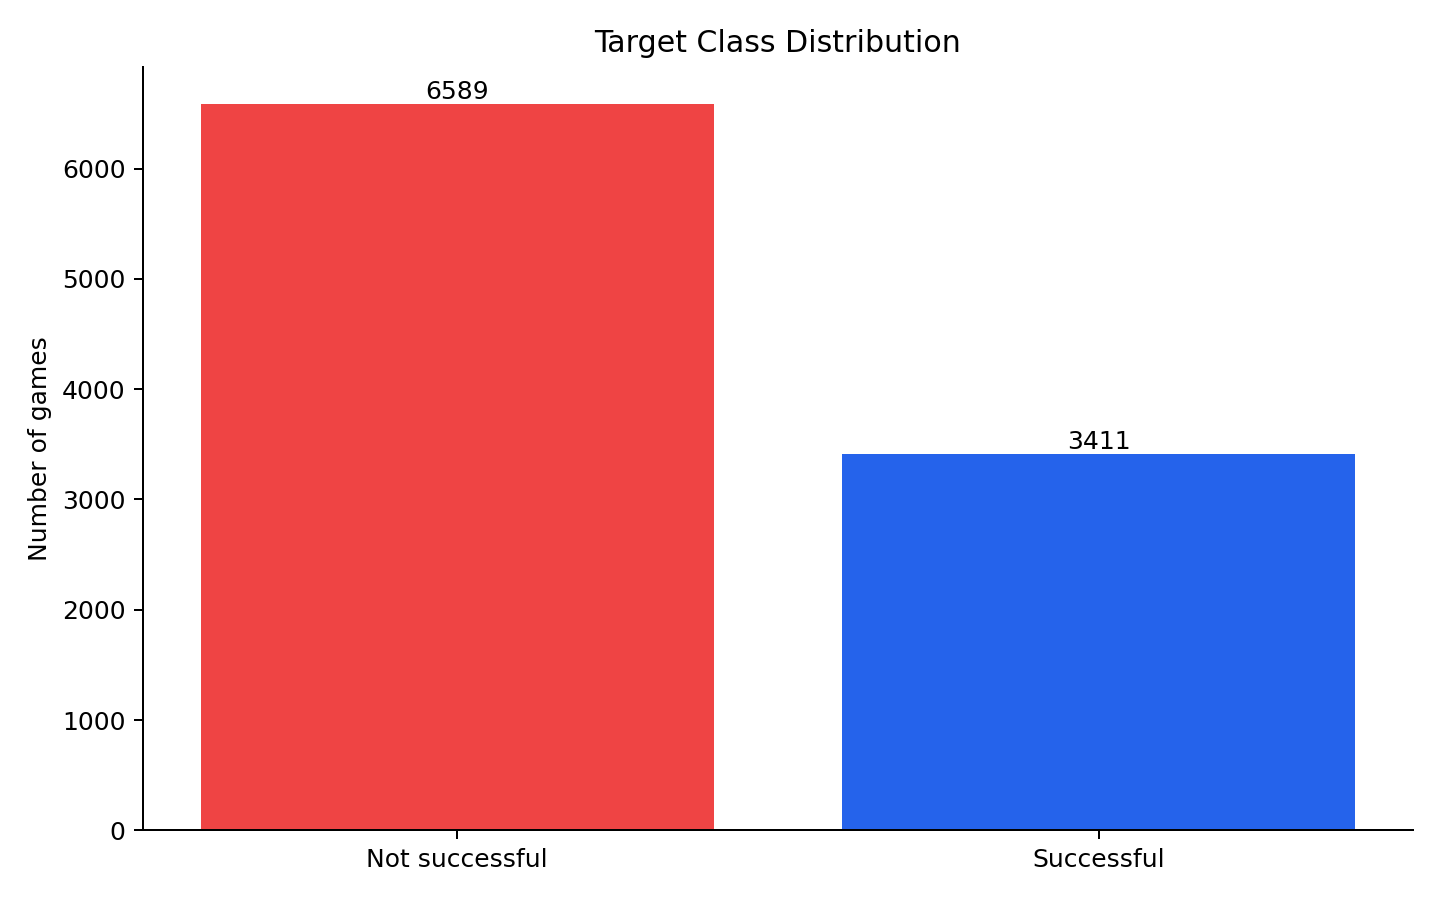
\includegraphics[width=0.8\textwidth]{target_distribution.png}
\caption{Target class distribution}
\label{fig:target-distribution}
\end{figure}

Figure~\ref{fig:notebook-target-preprocessing} shows the Jupyter Notebook code used to create the target variable and remove leakage-related columns before model training.

\begin{figure}[htbp]
\centering
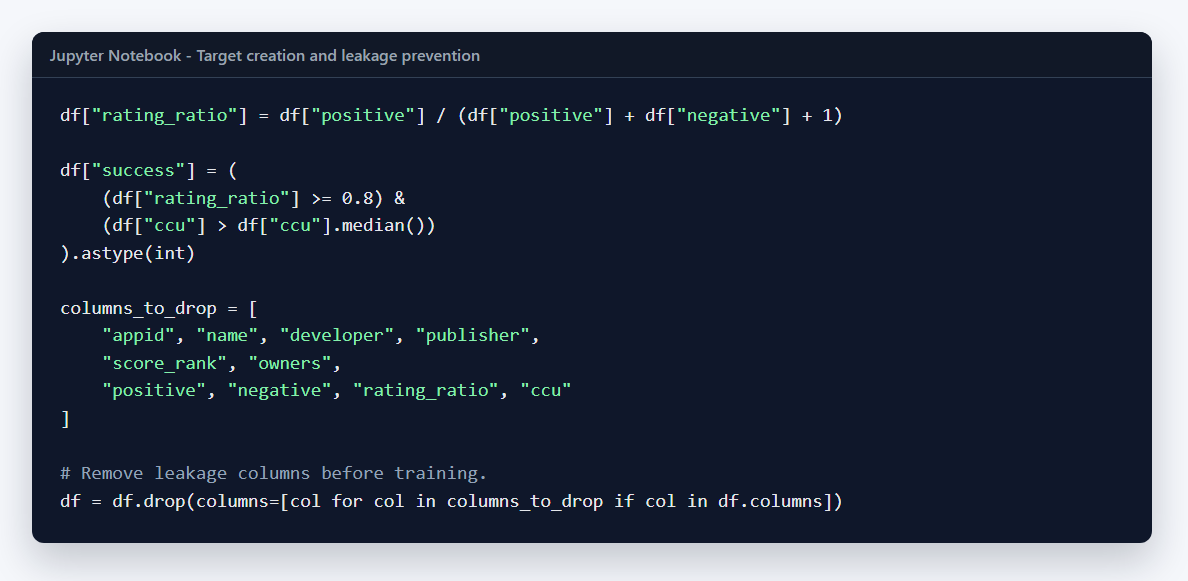
\includegraphics[width=0.95\textwidth]{notebook_target_preprocessing.png}
\caption{Notebook code for target creation and leakage prevention}
\label{fig:notebook-target-preprocessing}
\end{figure}

\section{Models}

\subsection{K-Nearest Neighbors}

KNN is a distance-based classification algorithm. It predicts the class of a new game by comparing it with the nearest games in the training data. Because KNN depends on distances, feature scaling is required.

Figure~\ref{fig:notebook-knn-code} shows the main KNN training and evaluation code from the Jupyter Notebook.

\begin{figure}[htbp]
\centering
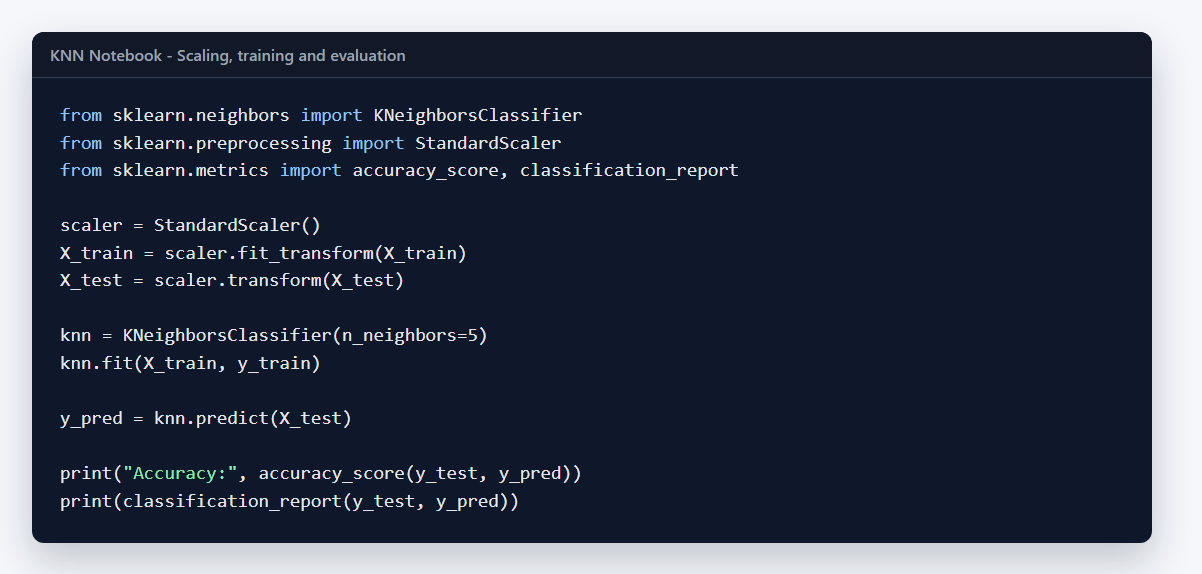
\includegraphics[width=0.95\textwidth]{notebook_knn_code.png}
\caption{KNN notebook training and evaluation code}
\label{fig:notebook-knn-code}
\end{figure}

\subsection{Support Vector Machine}

SVM tries to find the best decision boundary between successful and not successful games. The project uses an RBF kernel and balanced class weights.

Figure~\ref{fig:notebook-svm-code} shows the SVM training code. The RBF kernel is used, and \texttt{class\_weight="balanced"} helps handle class imbalance.

\begin{figure}[htbp]
\centering
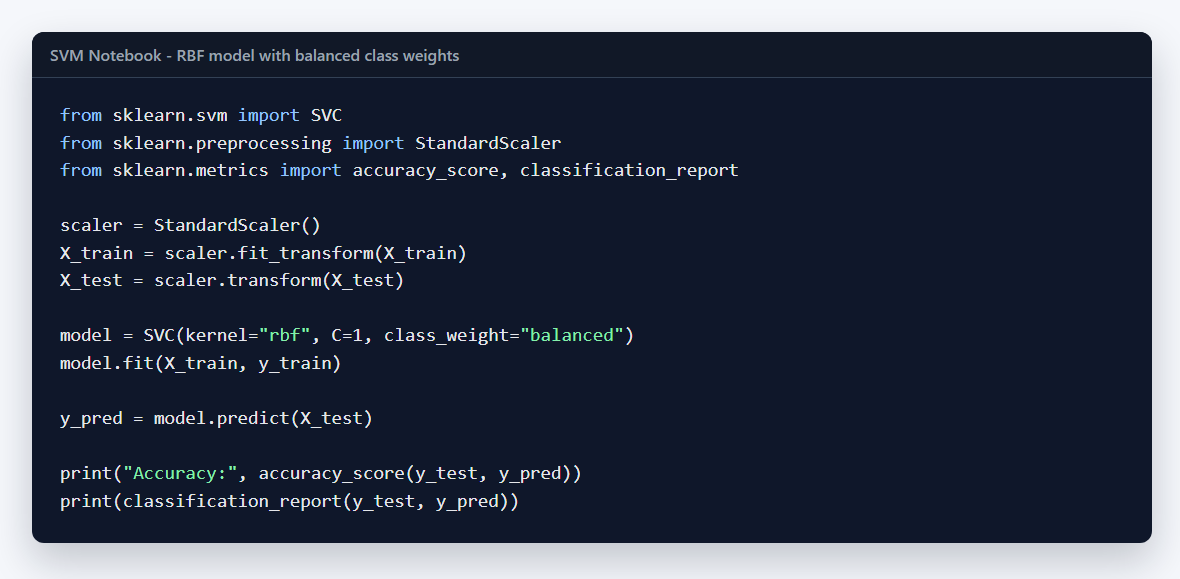
\includegraphics[width=0.95\textwidth]{notebook_svm_code.png}
\caption{SVM notebook training and evaluation code}
\label{fig:notebook-svm-code}
\end{figure}

\subsection{Random Forest}

Random Forest is an ensemble model based on many decision trees. It works well with tabular data and can handle non-linear relationships. It also provides feature importance values.

Figure~\ref{fig:notebook-rf-code} shows the Random Forest training and evaluation code, including the confusion matrix output.

\begin{figure}[htbp]
\centering
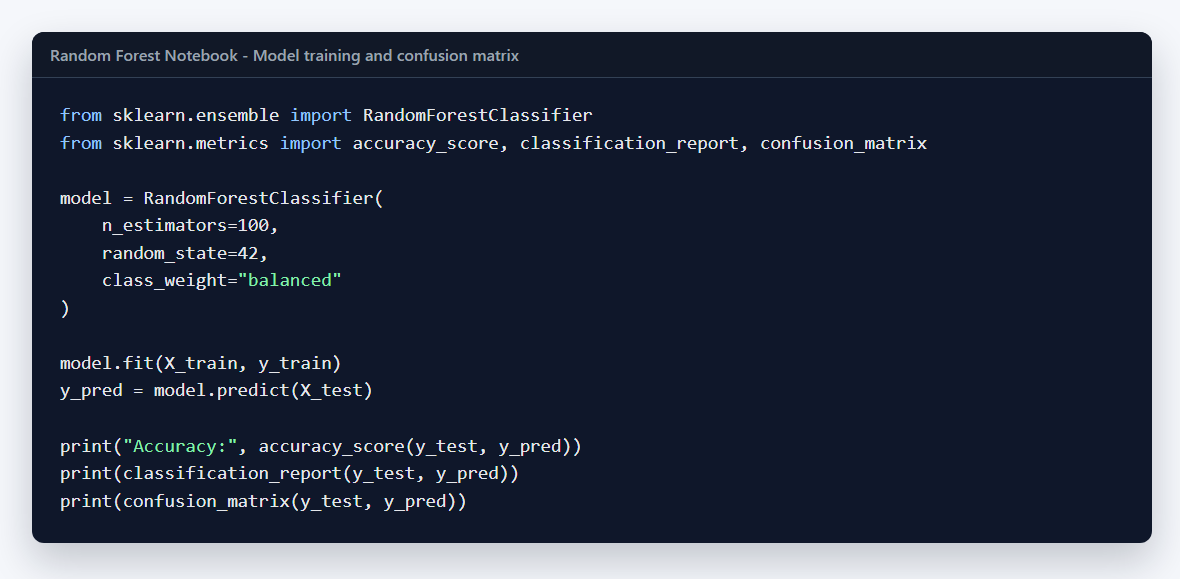
\includegraphics[width=0.95\textwidth]{notebook_random_forest_code.png}
\caption{Random Forest notebook training and evaluation code}
\label{fig:notebook-rf-code}
\end{figure}

\subsection{Deep Learning}

The Deep Learning model is a neural network built with TensorFlow/Keras. It uses dense layers and a sigmoid output layer for binary classification.

Figure~\ref{fig:notebook-dl-code} shows the neural network architecture and training configuration used in the Deep Learning notebook.

\begin{figure}[htbp]
\centering
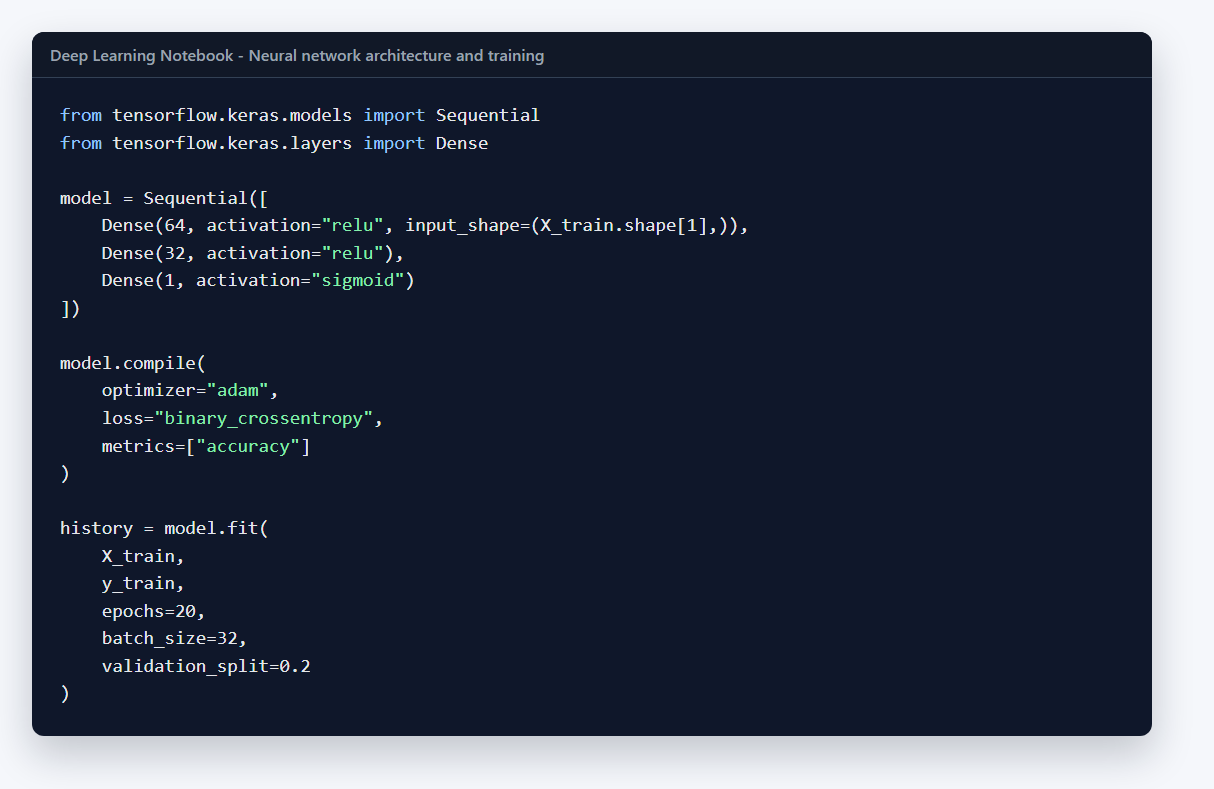
\includegraphics[width=0.95\textwidth]{notebook_deep_learning_code.png}
\caption{Deep Learning notebook architecture and training code}
\label{fig:notebook-dl-code}
\end{figure}

Figure~\ref{fig:dl-accuracy} shows the training and validation accuracy of the deep learning model across epochs. The validation accuracy remains close to the training accuracy, which indicates that the model learns useful patterns without a very large accuracy gap.

\begin{figure}[htbp]
\centering
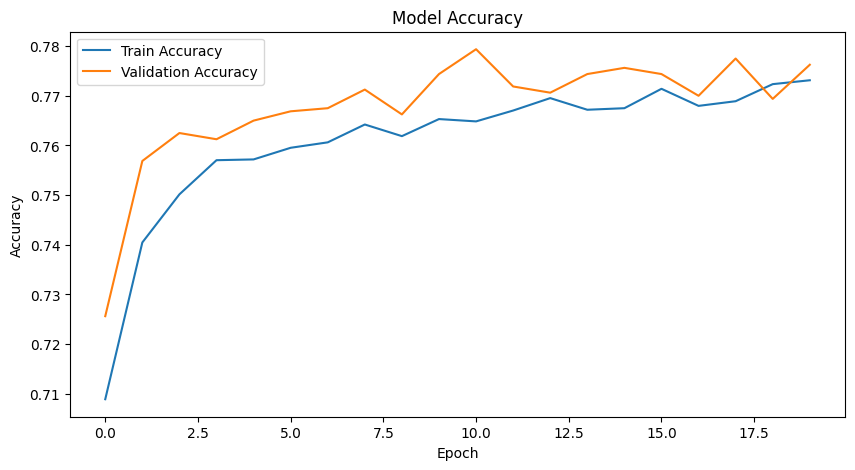
\includegraphics[width=0.85\textwidth]{deep_learning_training_1.png}
\caption{Deep Learning training and validation accuracy}
\label{fig:dl-accuracy}
\end{figure}

Figure~\ref{fig:dl-loss} shows the training and validation loss. The training loss continues to decrease, while the validation loss starts increasing after several epochs. This suggests that the model may begin to overfit after the earlier epochs.

\begin{figure}[htbp]
\centering
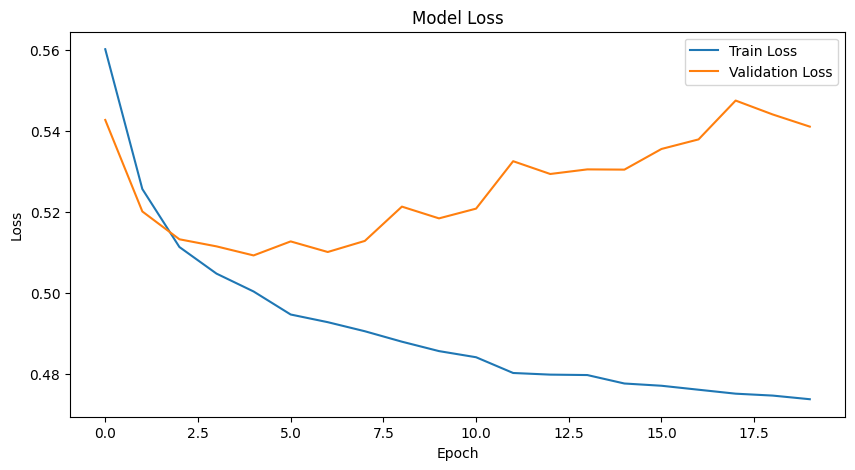
\includegraphics[width=0.85\textwidth]{deep_learning_training_2.png}
\caption{Deep Learning training and validation loss}
\label{fig:dl-loss}
\end{figure}

\section{Methodology}

The project follows a standard machine learning workflow. First, the Steam dataset is loaded and inspected. Then the target variable is created using review quality and player activity. After that, unnecessary text columns and leakage-related columns are removed. The cleaned data is split into training and test sets.

Figure~\ref{fig:workflow-diagram} summarizes the full workflow from the original dataset to the final Streamlit deployment.

\begin{figure}[htbp]
\centering
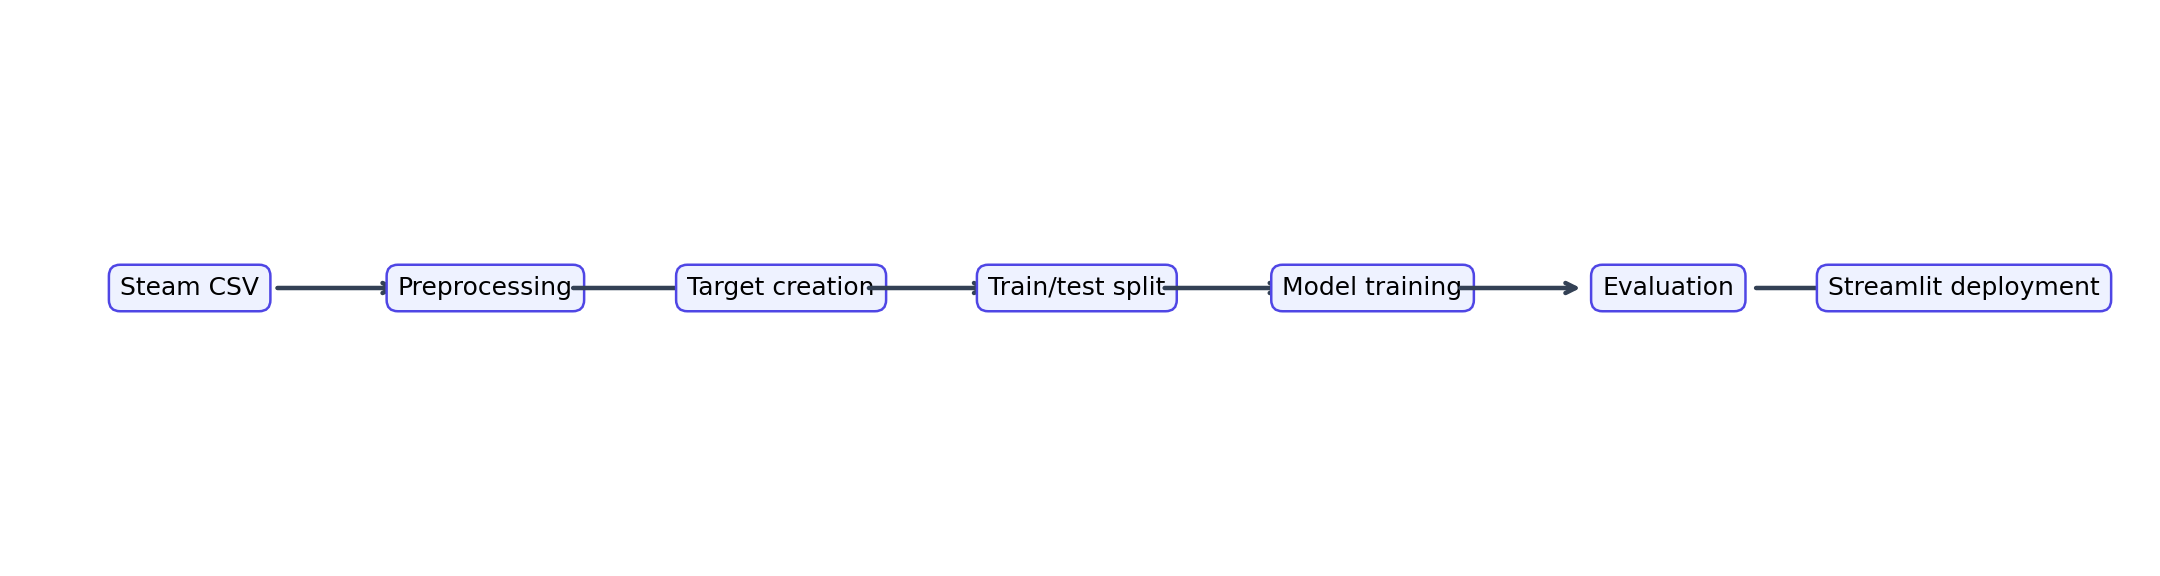
\includegraphics[width=\textwidth]{ml_workflow_diagram.png}
\caption{Machine learning workflow}
\label{fig:workflow-diagram}
\end{figure}

For KNN, SVM and Deep Learning, feature scaling is applied because these methods are sensitive to feature ranges. Random Forest does not require scaling because it is tree-based. Each model is trained, evaluated and saved to disk. The saved model files are then loaded by the Streamlit deployment application.

The methodology can be summarized as:

\begin{enumerate}[noitemsep]
    \item Load Steam dataset.
    \item Create \texttt{rating\_ratio} and \texttt{success} target.
    \item Remove text columns and leakage-related columns.
    \item Split data into training and test sets.
    \item Scale numerical features when required.
    \item Train KNN, SVM, Random Forest and Deep Learning models.
    \item Evaluate models using classification metrics.
    \item Apply cross-validation to classical models.
    \item Save trained models and preprocessing artifacts.
    \item Deploy models in Streamlit.
\end{enumerate}

\section{Preprocessing}

The preprocessing step removes text columns and unnecessary fields. For Random Forest and Deep Learning, leakage-related columns are also removed:

\begin{itemize}[noitemsep]
    \item \texttt{positive}
    \item \texttt{negative}
    \item \texttt{rating\_ratio}
    \item \texttt{ccu}
\end{itemize}

These columns are removed because they are directly related to the target variable. Keeping them would make the model performance unrealistically high.

\section{Evaluation}

The notebooks evaluate the models using:

\begin{itemize}[noitemsep]
    \item accuracy score
    \item classification report
    \item confusion matrix
    \item cross-validation
    \item mean cross-validation accuracy
    \item standard deviation of cross-validation accuracy
\end{itemize}

\subsection{Cross-Validation}

Cross-validation was added to the KNN, SVM and Random Forest notebooks. It evaluates a model across several data splits instead of only one train/test split.

\begin{lstlisting}[language=Python]
from sklearn.model_selection import cross_val_score

cv_scores = cross_val_score(model, X, y, cv=5, scoring="accuracy")

print("Cross-validation scores:", cv_scores)
print("Mean accuracy:", cv_scores.mean())
print("Standard deviation:", cv_scores.std())
\end{lstlisting}

For KNN and SVM, cross-validation is implemented with a \texttt{Pipeline} so that \texttt{StandardScaler} is fitted separately inside each fold. This prevents data leakage during validation.

\subsection{Standard Deviation}

The standard deviation shows how much the cross-validation results vary between folds. A lower standard deviation means that model performance is more stable.

\subsection{Results Summary}

Table~\ref{tab:results-summary} is prepared for final model comparison. The train/test results already exist in the notebooks. The cross-validation mean and standard deviation columns should be filled after running the new cross-validation cells in Jupyter Notebook.

\begin{table}[htbp]
\centering
\begin{tabular}{p{3.2cm} p{2.8cm} p{3.2cm} p{3.2cm}}
\toprule
\textbf{Model} & \textbf{Test Accuracy} & \textbf{CV Mean Accuracy} & \textbf{CV Std. Deviation} \\
\midrule
KNN & 0.782 & To be filled & To be filled \\
SVM & 0.561 & To be filled & To be filled \\
Random Forest & 0.759 & To be filled & To be filled \\
Deep Learning & 0.763 & Not applied & Not applied \\
\bottomrule
\end{tabular}
\caption{Model evaluation summary}
\label{tab:results-summary}
\end{table}

The Deep Learning model is not included in cross-validation because neural network cross-validation requires retraining the model several times, which is more computationally expensive than classical model validation.

Figure~\ref{fig:model-accuracy-comparison} visualizes the current test accuracy comparison between the four implemented models.

\begin{figure}[htbp]
\centering
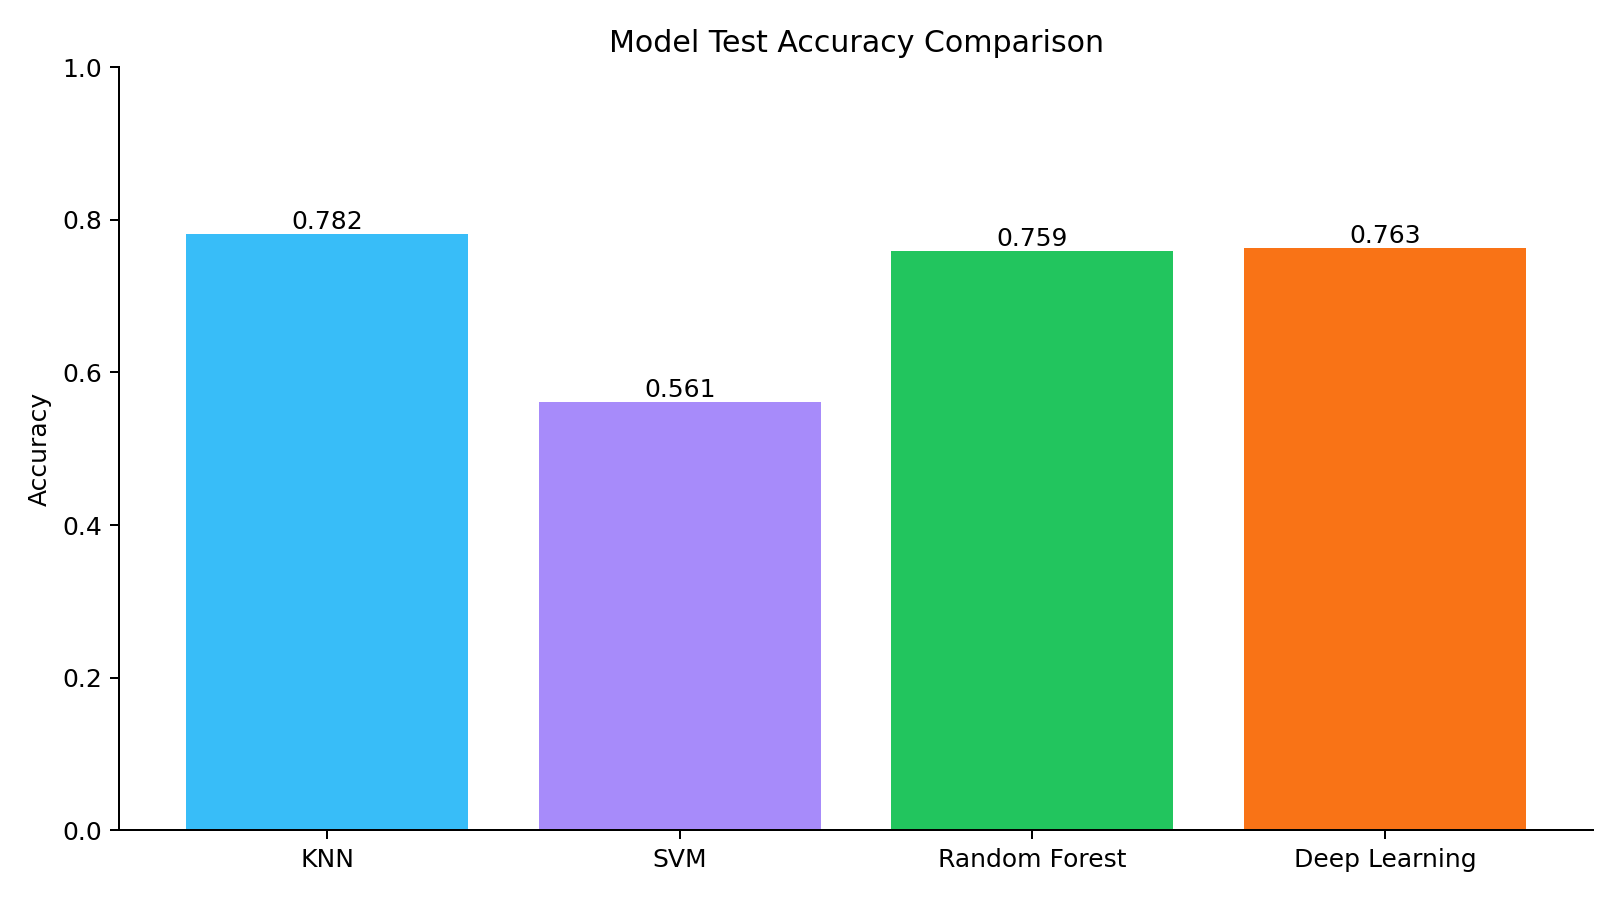
\includegraphics[width=0.85\textwidth]{model_accuracy_comparison.png}
\caption{Model test accuracy comparison}
\label{fig:model-accuracy-comparison}
\end{figure}

\subsection{Code Screenshots}

Figure~\ref{fig:code-cross-validation} shows the cross-validation code added to the classical machine learning notebooks. The output includes fold scores, mean accuracy and standard deviation.

\begin{figure}[htbp]
\centering
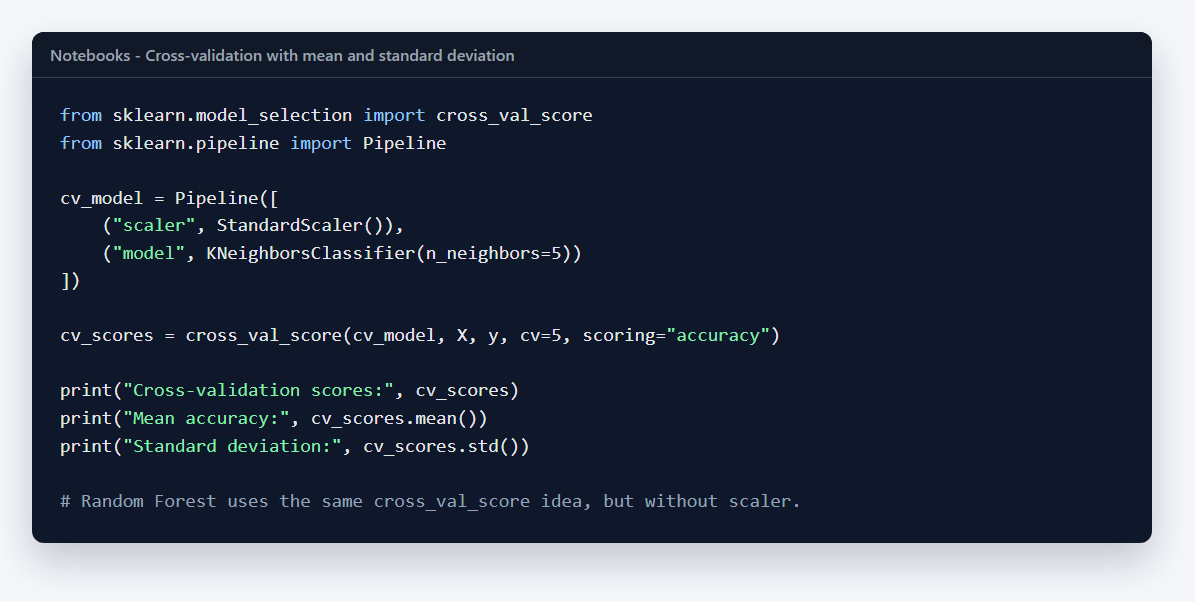
\includegraphics[width=0.95\textwidth]{code_cross_validation.png}
\caption{Cross-validation code with mean accuracy and standard deviation}
\label{fig:code-cross-validation}
\end{figure}

\section{Combined Streamlit Deployment}

The main deployment file is:

\begin{lstlisting}
D:\projects\app.py
\end{lstlisting}

This application loads all four trained models and compares their predictions in one interface.

The deployment is included as evidence that the trained models are not only evaluated in notebooks, but also integrated into a working user-facing application.

\subsection{Run Command}

Run the combined deployment from the root project folder:

\begin{lstlisting}[language=bash]
cd D:\projects
deepLearning\.venv\Scripts\python.exe -m streamlit run app.py
\end{lstlisting}

Then open:

\begin{lstlisting}
http://localhost:8501
\end{lstlisting}

\subsection{Deployment Features}

The combined app provides:

\begin{itemize}[noitemsep]
    \item one input form for all models
    \item prediction results for KNN, SVM, Random Forest and Deep Learning
    \item success probability or score for each model
    \item summary table
    \item successful game preset
    \item unsuccessful game preset
\end{itemize}

\subsection{Deployment Screenshots}

Figure~\ref{fig:streamlit-main-form} shows the combined Streamlit interface before prediction. The user can enter game information manually or use one of the preset example buttons.

\begin{figure}[htbp]
\centering
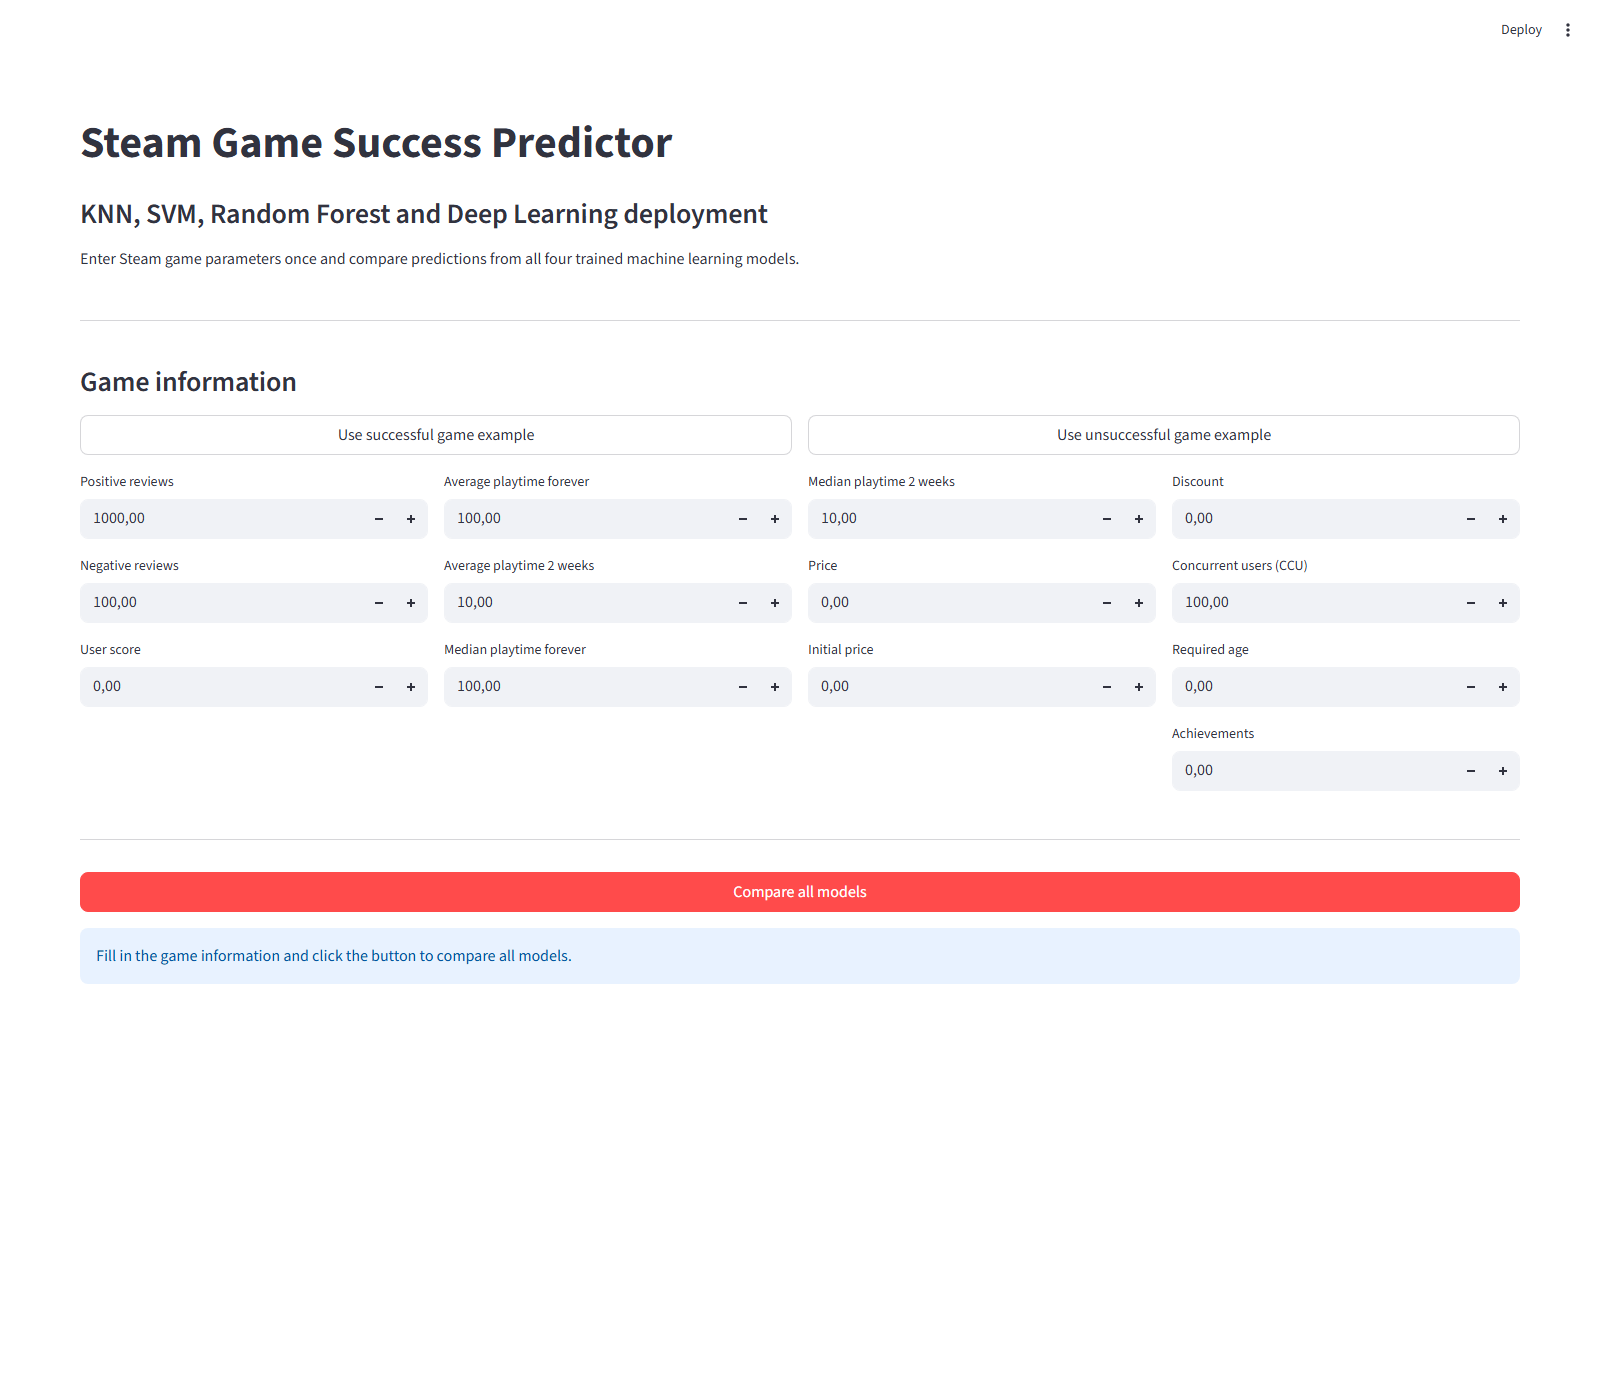
\includegraphics[width=0.95\textwidth]{streamlit_main_form.png}
\caption{Combined Streamlit deployment input form}
\label{fig:streamlit-main-form}
\end{figure}

Figure~\ref{fig:streamlit-successful} shows the successful game preset. In this example, all four models predict that the game is successful.

\begin{figure}[htbp]
\centering
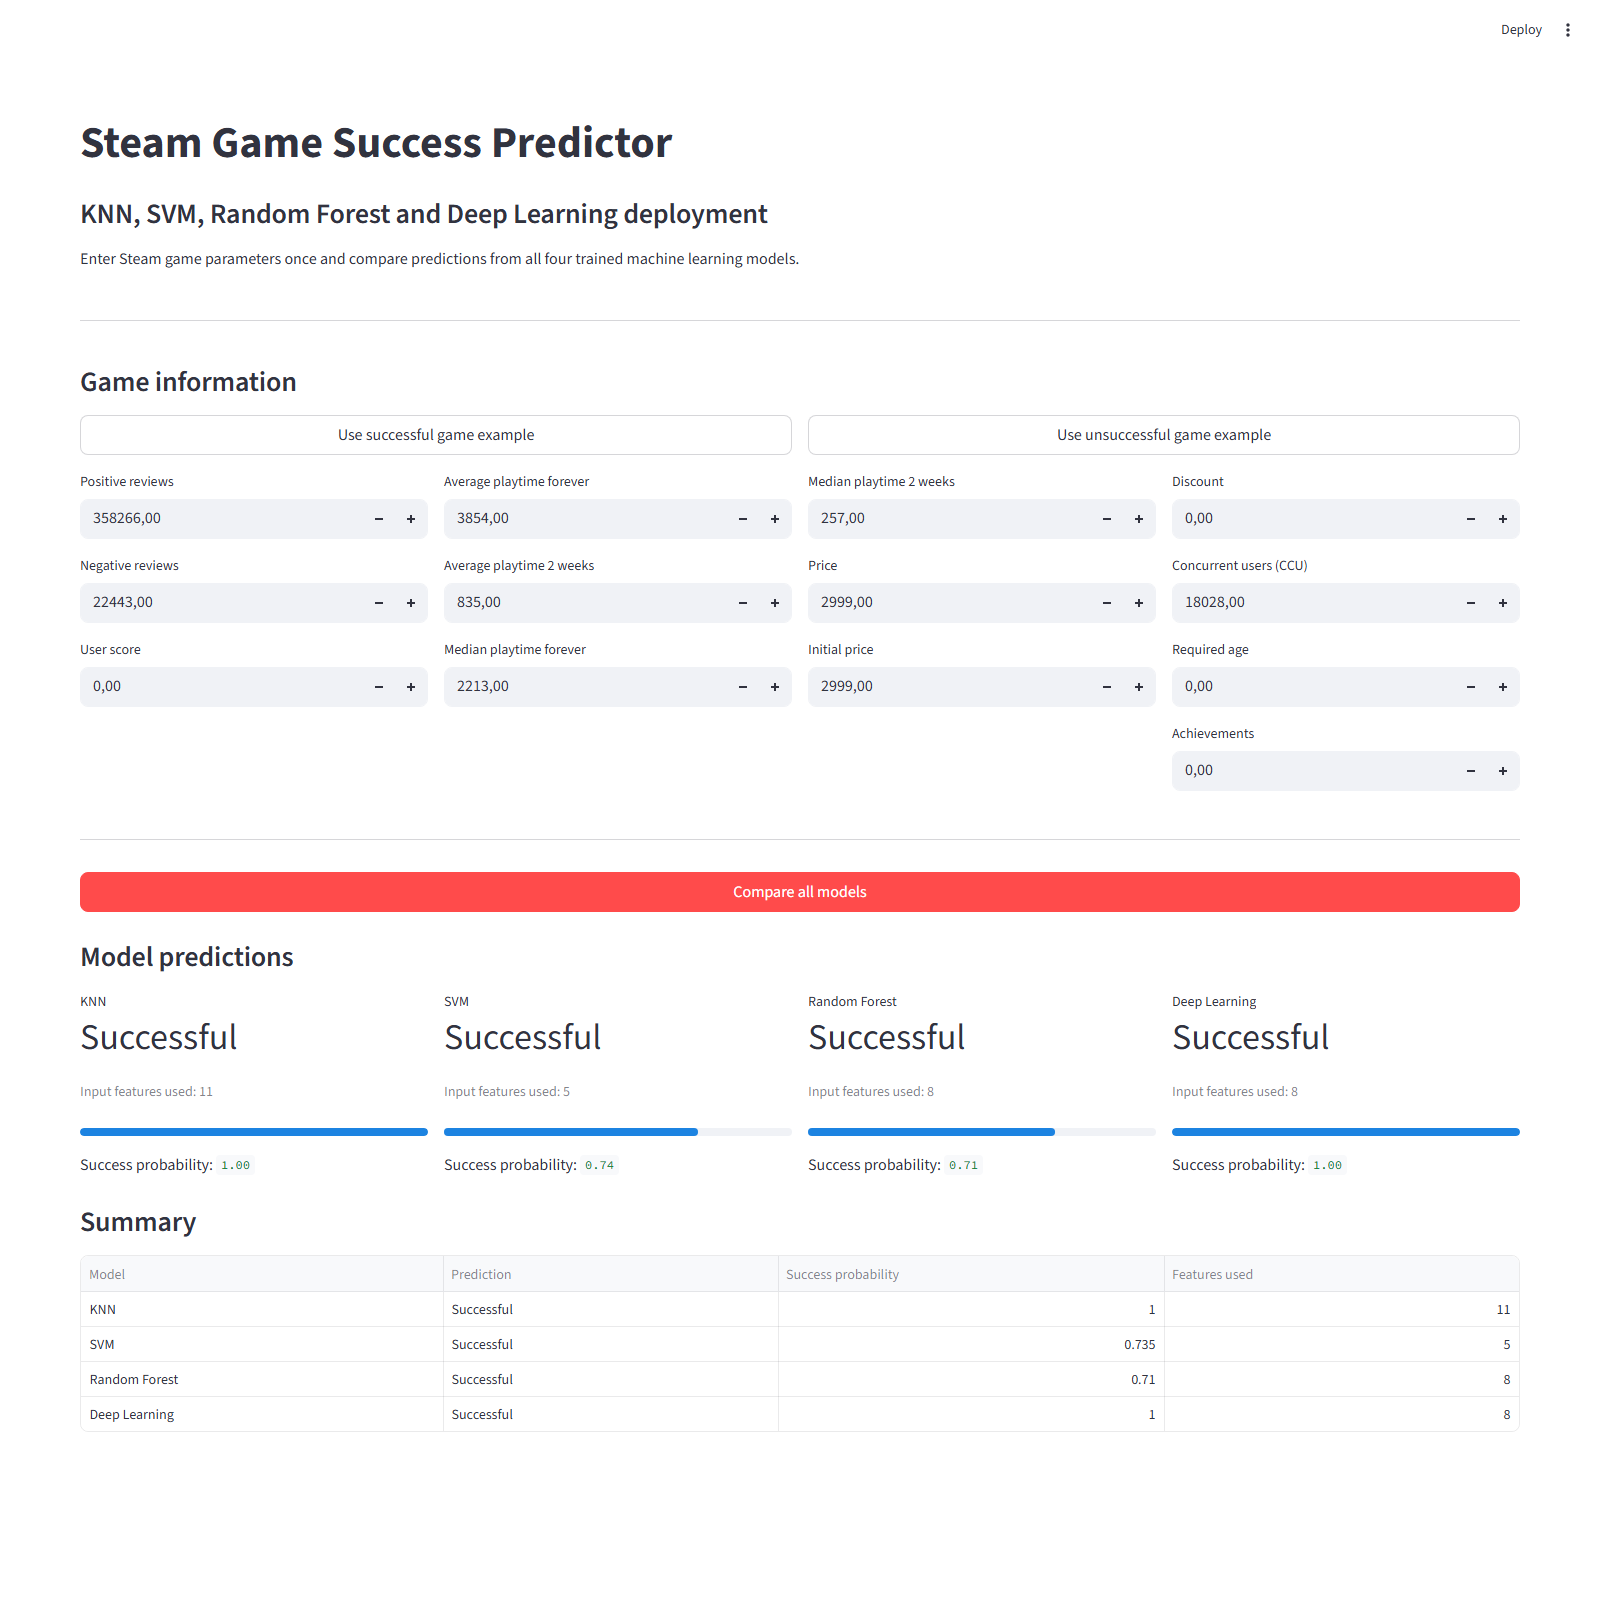
\includegraphics[width=0.95\textwidth]{streamlit_successful_prediction.png}
\caption{Successful game example prediction results}
\label{fig:streamlit-successful}
\end{figure}

Figure~\ref{fig:streamlit-unsuccessful} shows the unsuccessful game preset. In this example, all four models predict that the game is not successful.

\begin{figure}[htbp]
\centering
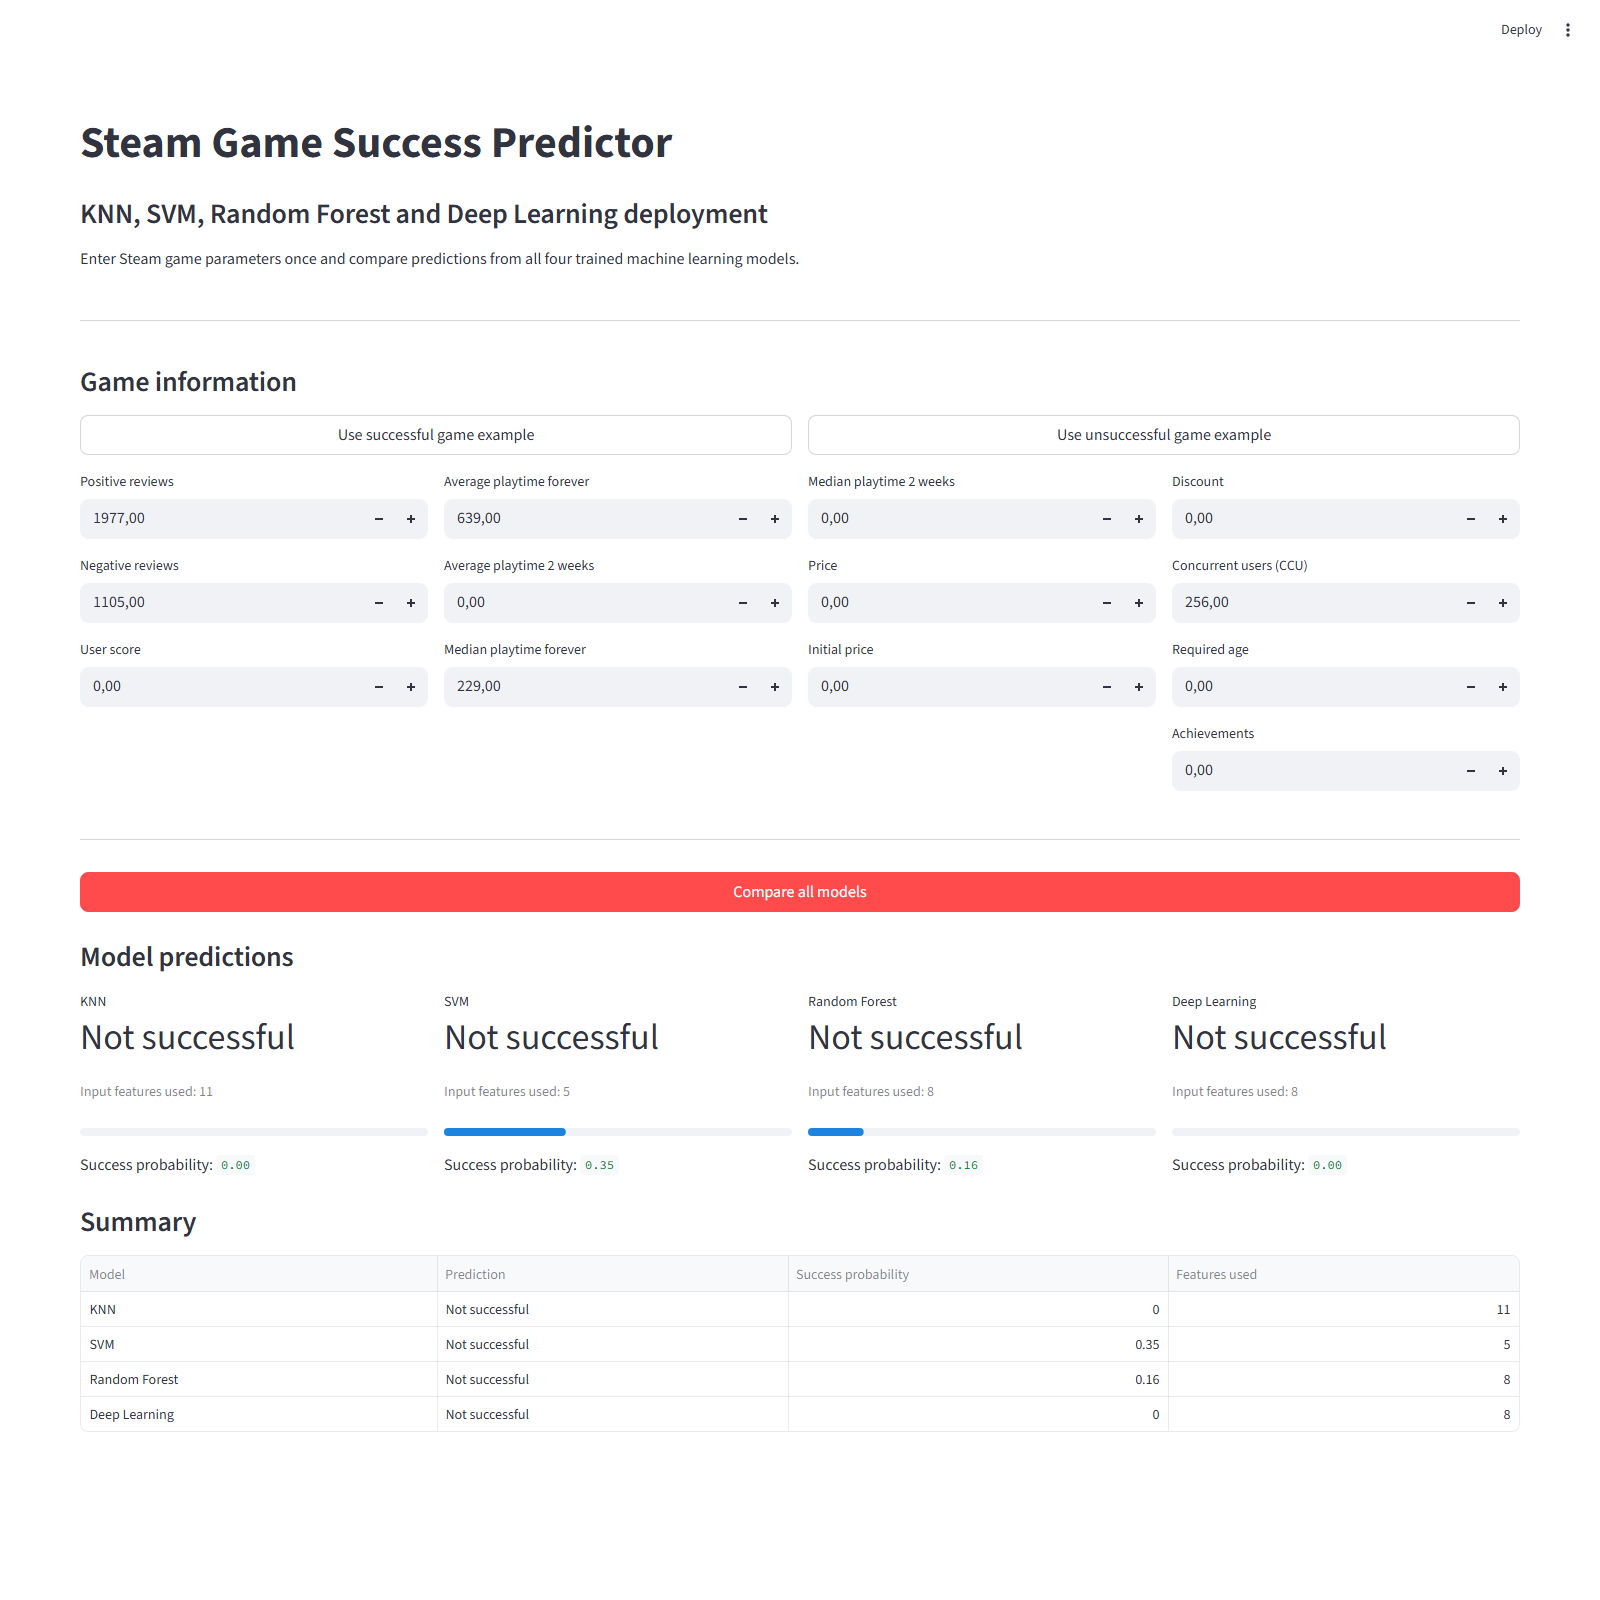
\includegraphics[width=0.95\textwidth]{streamlit_unsuccessful_prediction.png}
\caption{Unsuccessful game example prediction results}
\label{fig:streamlit-unsuccessful}
\end{figure}

\subsection{Deployment Code Screenshots}

Figure~\ref{fig:code-model-loading} shows how the combined Streamlit application loads the saved model files, scalers and feature lists from the individual project folders.

\begin{figure}[htbp]
\centering
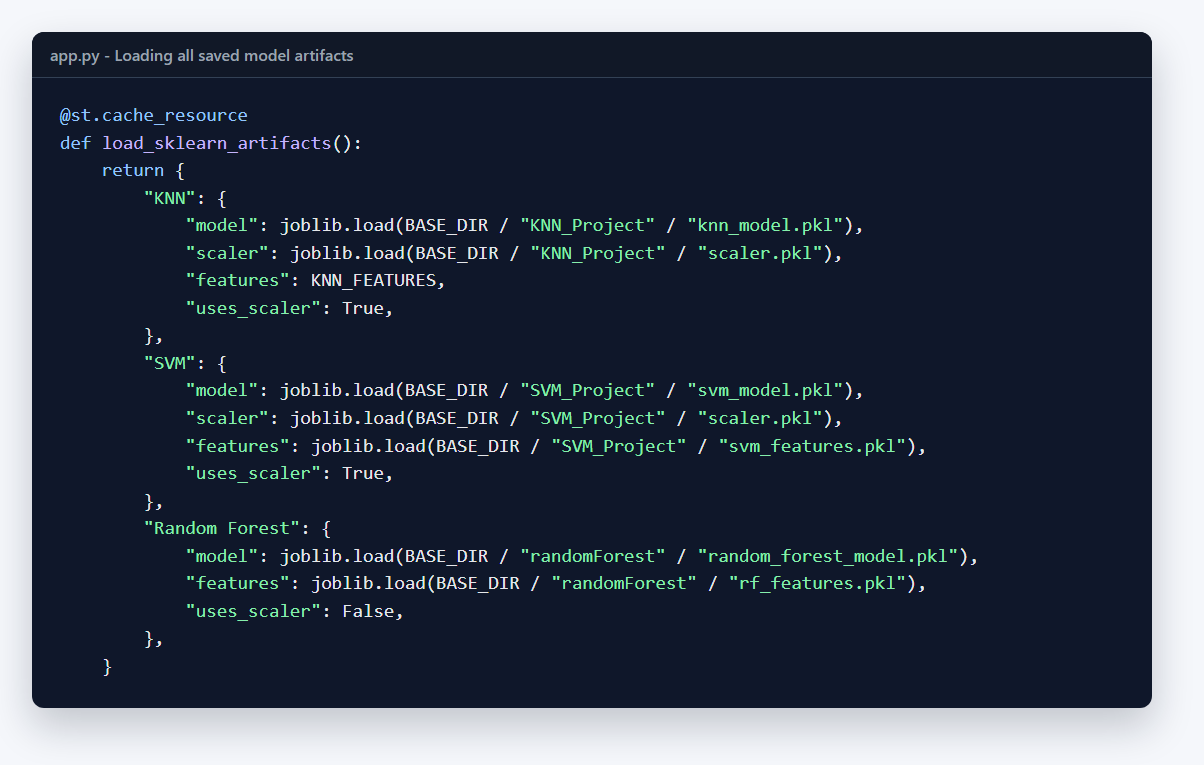
\includegraphics[width=0.95\textwidth]{code_combined_deployment.png}
\caption{Combined deployment model loading code}
\label{fig:code-model-loading}
\end{figure}

Figure~\ref{fig:code-prediction-logic} shows the prediction logic used by the combined Streamlit application. For SVM, the application uses \texttt{decision\_function} because the saved SVM model was trained without \texttt{probability=True}.

\begin{figure}[htbp]
\centering
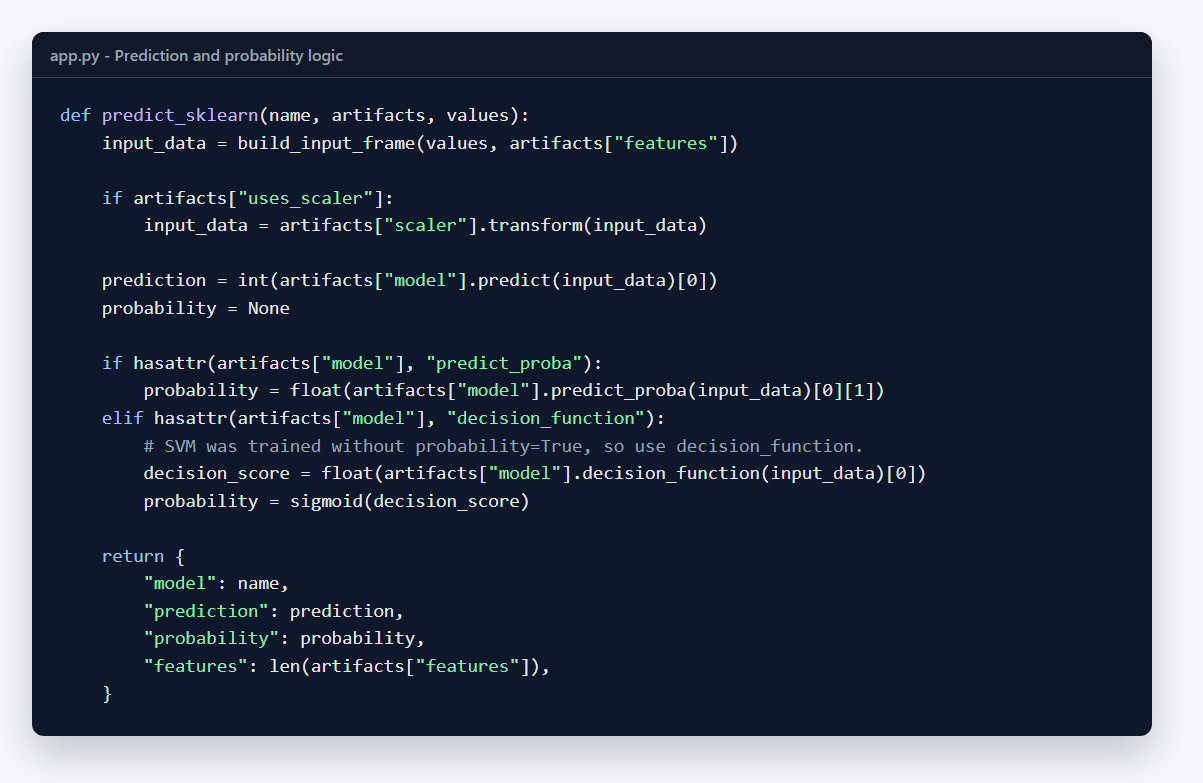
\includegraphics[width=0.95\textwidth]{code_prediction_logic.png}
\caption{Prediction and probability logic in the combined app}
\label{fig:code-prediction-logic}
\end{figure}

\subsection{Preset Buttons}

The app includes two buttons for demonstration:

\begin{itemize}[noitemsep]
    \item \texttt{Use successful game example}
    \item \texttt{Use unsuccessful game example}
\end{itemize}

These buttons fill the input fields with example values from the dataset. The successful preset is selected so that all four models predict \texttt{Successful}. The unsuccessful preset is selected so that all four models predict \texttt{Not successful}.

\section{Individual Streamlit Apps}

Each model also has a separate Streamlit app.

\subsection{KNN}

\begin{lstlisting}[language=bash]
cd D:\projects\KNN_Project
..\deepLearning\.venv\Scripts\python.exe -m streamlit run app.py
\end{lstlisting}

\subsection{SVM}

\begin{lstlisting}[language=bash]
cd D:\projects\SVM_Project
..\deepLearning\.venv\Scripts\python.exe -m streamlit run app.py
\end{lstlisting}

\subsection{Random Forest}

\begin{lstlisting}[language=bash]
cd D:\projects\randomForest
..\deepLearning\.venv\Scripts\python.exe -m streamlit run app.py
\end{lstlisting}

\subsection{Deep Learning}

\begin{lstlisting}[language=bash]
cd D:\projects\deepLearning
.venv\Scripts\python.exe -m streamlit run app.py
\end{lstlisting}

\section{Required Saved Files}

\begin{table}[h]
\centering
\begin{tabular}{p{4cm} p{9cm}}
\toprule
\textbf{Project} & \textbf{Required Files} \\
\midrule
KNN & \texttt{knn\_model.pkl}, \texttt{scaler.pkl} \\
SVM & \texttt{svm\_model.pkl}, \texttt{scaler.pkl}, \texttt{svm\_features.pkl} \\
Random Forest & \texttt{random\_forest\_model.pkl}, \texttt{rf\_features.pkl} \\
Deep Learning & \texttt{deep\_learning\_model.keras}, \texttt{dl\_scaler.pkl}, \texttt{dl\_features.pkl} \\
\bottomrule
\end{tabular}
\caption{Required saved files}
\end{table}

\section{How to Update Model Files}

If a notebook is rerun, saved model files may be overwritten by \texttt{joblib.dump()} or \texttt{model.save()}. This is normal and does not require deleting old files manually.

If only cross-validation results are needed, the saved model files do not need to be deleted.

\section{Known Notes}

\begin{itemize}[noitemsep]
    \item Deep Learning cross-validation is not included because it is slower and more complex than classical model cross-validation.
    \item SVM was trained without \texttt{probability=True}. In the combined app, its score is estimated using \texttt{decision\_function}.
    \item The root deployment app depends on the saved model files in all project folders.
    \item The virtual environment is located in \texttt{deepLearning/.venv}.
\end{itemize}

\section{Limitations}

The project has several limitations:

\begin{itemize}[noitemsep]
    \item The dataset uses available Steam numerical features, but it does not fully capture marketing, genre popularity, release timing or external trends.
    \item The target variable is manually defined using review ratio and concurrent users, so it is an approximation of real commercial success.
    \item SVM probability is estimated in the combined app using \texttt{decision\_function}, because the saved SVM model was not trained with \texttt{probability=True}.
    \item Deep Learning cross-validation is not included due to additional training time.
    \item Some models use different feature sets because leakage columns were removed from the improved models.
\end{itemize}

\section{Future Improvements}

Future work could improve the project in the following ways:

\begin{itemize}[noitemsep]
    \item add hyperparameter tuning with \texttt{GridSearchCV} or \texttt{RandomizedSearchCV};
    \item retrain SVM with \texttt{probability=True} for calibrated probability output;
    \item add ROC-AUC and precision-recall curve analysis;
    \item include more features such as genres, release date and tags;
    \item use a unified feature set across all models;
    \item add model explainability with feature importance or SHAP values;
    \item deploy the Streamlit application online.
\end{itemize}

\section{Conclusion}

The project demonstrates a complete machine learning workflow: data preparation, target creation, model training, evaluation, cross-validation and deployment. The combined Streamlit app makes it possible to compare KNN, SVM, Random Forest and Deep Learning predictions in one interface.

\end{document}
